\documentclass[10pt]{article}
\usepackage[utf8]{inputenc}
\usepackage[spanish]{babel}
%\usepackage{nopageno}
\usepackage[top=2cm,bottom=2.5cm,left=1.5cm,right=1.5cm]{geometry}

% Fuente Times New Roman
\usepackage{newtxtext,newtxmath}
% Columns Layout
\usepackage{multicol}
% Dummy text
\usepackage{blindtext}
% Justificar texto
\usepackage{ragged2e}
% Packages for tables
\usepackage{longtable}
% Images
\usepackage{graphicx}
% Minipages captions
\usepackage{caption}
\captionsetup{
	font=small,
	labelfont=bf,
	tableposition=top,
	width=0.72\columnwidth,
	justification=raggedright
}
% Enum configurations
\usepackage{enumitem}
% Multiple rows in tables
\usepackage{multirow}


\begin{document}
	
	\begin{center}
	\vspace*{2.3cm}
	
	%{\LARGE \textbf{Clasificador de gestos motrices para la creación de texto utilizando vectores de atributos SAX-DTW}}
	{\LARGE \textbf{Clasificador de gestos motrices utilizando vectores de atributos distancia DTW sobre series de tiempo en representación SAX}}
	
	\vspace{0.5cm}
	
	{\large Eduardo Valle}
	
	\vspace{0.1cm}
	
	{\large \textit{Escuela Superior de Cómputo}}
	
	\vspace{0.1cm}
	
	{\large \textit{Instituto Politécnico Nacional}}
	
	\vspace{0.1cm}
	
	{\large Ciudad de México, México}
	
	\vspace{0.1cm}
	
	{\large lvalle212@gmail.com}
	
\end{center}

	\begin{multicols}{2}
		
		{\small
			\justifying
			\textbf{\textit{Resumen}--- Este trabajo presenta un análisis de la efectividad en términos de precisión y tiempo de ejecución, para 3 modelos que implementan el algoritmo DTW, la técnica SAX y modelos clásicos de \textit{machine learning} como \textit{k-NN} y \textit{SVC}, en la tarea de clasificación de series de tiempo. Bajo el contexto de reconocimiento de gestos motrices, se utilizan patrones en términos de fuerzas de aceleración, muestreados en los ejes tridimensionales usando el sensor acelerómetro integrado en dispositivos \textit{wearable} o \textit{smartphones}. Se analiza el desempeño de los modelos con el conjunto de datos \textit{Gesture Pebble}, publicamente disponible en \textit{UCR Time Series Archive}, que se compone por 304 patrones procedente de 4 participantes distintos, representados como series de tiempo de longitud variable de las mediciones de la acelaración en el eje Z para 6 gestos únicos.}
			
			\hfill\break
			\justifying
			\textbf{\textit{Términos Clave}--- Clasificación de series de tiempo, \textit{Dynamic Time Warping}, \textit{Symbolic Aggregate Approximation}}
		}
		
		\hfill\break
		\centering
		I. ~~~~~~ INTRODUCCIÓN
		
		\hfill\break
\justifying
Las afecciones del habla e impedimentos en la expresión oral en adultos mayores suele originarse después de haber sufrido una lesión por traumatismo craneoecenfálico o un accidente cerebrovascular que daña principalmente el lóbulo izquierdo del cerebro, derivando principalmente en 3 condiciones médicas, las afasias[1], apraxias[2] y disartrias[3]. Estos tipos de afectaciones al habla resultan en alteraciones del lenguaje, pérdida de la capacidad para la realización de gestos diestros aún cuando se mantiene el deseo y capacidad física de hacerlos, y trastornos en la ejecución motora del habla.

\hfill\break
\justifying
En el contexto de esta problemática se plantea un alternativa de solución como una propuesta que tiene por objetivo la creación de una herramienta embebida de apoyo a la comunicación verbal para pacientes en estas condiciones, permitíendoles conformar palabras y texto mediante la replicación de gestos con una mano pertenecientes a un código motriz, desarrollado específicamente para esta solución, que describen a letras del alfabeto y son repducidos sonoramente mediante el uso de un servicio de texto a voz. El desarrollo de la solución se planea como tema de trabajo de titulación a nivel licenciatura para la Ingeniería de Ciencias Computacionales en la Escuela Superior de Computación.

\hfill\break
\justifying
De esta solución compete a este documento, el desarrollo de la técnica algorítmica encargada de realizar la tarea de clasificación de los gestos motrices como series dependientes del tiempo, a sus clases alfabéticas. Trabajando en este marco contextual, se toman algunas consideraciones durante la elección del conjunto de datos prueba y el desarrollo experimental, derivado de la guía principal en este trabajo: La replicación de las condiciones bajo las que se desarrollará el proyecto solución con la mayor proximidad posible.

\hfill\break
\justifying
Las condiciones de la solución involucran la creación particular de un conjunto de datos con los gestos del código motriz, pendiente de definición en el momento en el que se produce este trabajo, utilizando únicamente el sensor acelerómetro para el muestreo de las fuerzas en los ejes tridimensionales para su uso como instancias de entrenamiento del modelo clasificador. 

\hfill\break
\justifying
También tomando relevancia en la elección y análisis de las técnicas algorítmicas evaluadas experimentalmente, aparece la condicionante de los recursos computacionales disponibles en un contexto embebido donde la mayor capacidad de cálculo se concentra en un SoC RaspberryPi 3B+, enfatizando la necesidad de algoritmos de baja complejidad, comparando como ejemplo con alguna solución que involucre redes neuronales o técnicas de \textit{Deep Learning}, que provean resultados de alta precisión sin un gran costo computacional y temporal.
		
		\hfill\break
		\centering
		II. ~~~~~~ TRABAJOS RELACIONADOS
		
		
\hfill\break
\justifying
La inherente naturaleza descriptiva con una noción de ordenamiento, especificamente temporal, de las series de tiempo, les mantiene presente en casi cualquier tarea que involucra un proceso cognitivo humano[4], muchos otros fenómenos recurrentes en la naturaleza y cantidad de ámbitos de interes humano como negocios, economía, ingeniería, medio ambiente, medicina y otras áreas de investigación científica que recolectan datos en forma de secuencias dependientes del tiempo[5].

\hfill\break
\justifying
La tarea de clasificación de series temporales o \textit{Time Series Classification}(TSC), consiste en el entrenamiento de un clasificador en un conjunto de entradas de entrenamiento en unos casos específicos, en donde cada caso contiene un conjunto ordenado de atributos en valores reales y una etiqueta de clase[6]. Se trata de un tema ampliamente estudiado y de gran interés en un extenso rango de áreas como \textit{data mining}, estadística, procesamiento de señales, ciencias ambientales, bilogía computacional, procesamiento de imágenes, quimiometría, etc[6]. Representando tal importancia e influencia, que cualquier problema de clasificación que utiliza datos registrados tomando en consideración una noción de ordenamiento, puede ser transformado a un problema de TSC[4].

\hfill\break
\justifying
Con los años, investigadores han invertido un gran esfuerzo en estudios para el desarrollo de modelos que resuelvan el problema planteado por TSC y cada vez con una mayor precisión. Con la creciente disponibilidad de datos temporales[4] y archivos como \textit{UCR Time Series Archive}[7], ha desencadenado el crecimiento en el número de algoritmos propuestos para TSC, implementando técnicas que utilizan modelos de \textit{Machine Learning} y diferentes medidas de distancia, técnicas para la transformaciones del espacio de los datos[6], técnicas de \textit{ensembling}(entrenamiento de un conjunto de modelos menores que integrando sus salidas resultan en un mejor modelo)[8], hasta nuevas alternativas de modelos \textit{Deep Learning}, en la tendencia para muchas áreas de la IA, con un influencia relativamente nueva pero creciente en lo referente al problema de TSC[4].

\hfill\break
\justifying
Refiriendo a la problemática, la solución embebida como herramienta de apoyo a la comunicación verbal para personas con afecciones del habla, existen cantidad de artículos, \textit{papers} y proyectos que funcionan como estado de arte a la solución pero con un contraste importante en los objetivos entre este trabajo. La principal necesidad que atienden los trabajos[9,10,11,12] es la implementación de una solución tecnológica que se enfoca en traducir el lenguaje de señas del respectivo país, a discurso hablado, pero escencialmente las circunstancias en las que se plantean las problemáticas con este trabajo son distintas. La solución propuesta cuenta con un contexto muy distinto en el concepto de la traducción, implementando el código motriz como principal conjunto símbolico, particular y único a la solución, mostrando evidente la diferencia con la extendida población que comunica el lenguaje de señas.

\hfill\break
\justifying
Otro punto de constraste se encuentra en el ámbito de implementación y usuarios objetivos. Las tecnologías del estado de arte sirve para comunicar desde la comunidad con dominio en el lenguaje de señas, hacia la sociedad general en un contexto cotidiano. La solución que se propone en cambio, se muestra circunstancial pues funciona como herramienta de primer contacto con pacientes que han sufrido recientemente el accidente o lesión, y son incapaces de comunicarse pero en sus condiciones previas no se encontraban limitados en la expresión oral.

\hfill\break
\justifying
Enfocandose principalmente en el objetivo que atiende este artículo, el problema de TSC para gestos motrices, se distingue un \textit{paper} que atiende en profundidad y de manera particular, la identificación de gestos motrices utilizando un sensor acelerómetro para el muestreo de las fuerzas en los 3 ejes durante la ejecución del patrón con una mano[13]. En el trabajo Mezari y Maglogiannis, utiliza un \textit{smartwatch} Pebble como elemento sensor, exponiendo el objetivo del trabajo como una examinación del uso de dispositivos básicos como \textit{smartphones} y \textit{wearables}, para el reconocimiento confiable de gestos simples y naturales, proponiendo además una metodología para mejorar el desempeño y precisión.
		
		\hfill\break
		\centering
		III. ~~~~~~ DESCRIPCIÓN DEL CONJUNTO DE DATOS
		
		
\hfill\break
\justifying
Manteniendo en mente las condiciones del proyecto, se eligió a corde un conjunto de datos para el entrenamiento y prueba de los métodos experimentados. El conjunto de datos elegido \textit{GesturePebble}, se deriva del trabajo \textit{"Gestures Recognition using Symbolic Aggregate Aproximation and Dynamic Time Warping on Motion Data"}[13], el conjunto de datos se encuentra disponible para su uso público en el repositorio de series temporales \textit{UCR Archive}[7].

\hfill\break
\justifying
Incluye instances de series temporales con longitud varible, razón por la que el archivo provisto por UCR, se encuentra acompletado a una longitud de 456 mediciones por patrón con el uso de NaNs en las instancias con menor longitud. Así mismo las etiquetas de clase se colocan como el primer elemento de cada secuencia para un fácil manejo.

\hfill\break
\justifying
Enfocado en el estudio de dispositivos cotidianos como celulares y \textit{wearables} para el reconocimiento de gestos, los datos recolectados son muestreados con las mediciones ofrecidas por el acelerómetro del reloj inteligente Pebble, en los ejes tridimensionales al ser utilizado sobre la muñeca por los sujetos participantes en la generación del conjunto de datos.

\hfill\break
\justifying
El \textit{dataset} involucra a 4 participantes, cada uno instruido para realizar 6 gestos(Figura 1) que repitieron durante un par de sesiones separadas entre días para conseguir un total de 8 grabaciones y completo el \textit{dataset} a un total de 304 gestos. 

\hfill\break
\begin{minipage}{\linewidth}
	\centering
	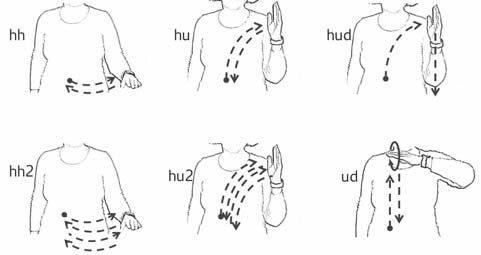
\includegraphics[width=7.5cm]{Imagenes/gestos_motrices.png}
	\label{gestos_motrices}
	\captionof{figure}{Elección de los 6 gestos sencillos etiquetados y realizados por los participantes para la generación de las secuencias temporales disponibles en el \textit{dataset} \textit{GesturePebble}}
\end{minipage}

\hfill\break
\justifying
De las series temporales captadas, se proveén las mediciones del sensor acelerómetro en el eje Z únicamente, facilitando a su vez un par de conjutos de datos con características específicas cada uno: \textit{GesturePebbleZ1} y \textit{GesturePebbleZ2}.

\hfill\break
\justifying
El conjunto de datos \textit{GesturPebbleZ1}, provee un archivo con instancias para el entrenamiento del modelo clasificador, componíendose los patrones desarrollados por los partipantes durante la primer sesión. Mientras que el archivo de prueba, es la colección de los patrones realizados en la segunda sesión.

\hfill\break
\justifying
Para el conjunto \textit{GesturePebbleZ2}, el conjunto de entrenamiento consiste en los datos de un par de sujetos, y el de prueba del par restante. Presumiblemente esta segunda colección está destinado a ser más compleja en dificultad que el primero, impidiendo que el modelo sea entrenado con patrones de los sujetos que más tarde serán evaluados. La dificultad de este \textit{dataset} se argumenta basándose en el hecho de que cada participante posé una postura y mecánica de movimiento distinta a las de los demás.
		
		\hfill\break
		\centering
		IV. ~~~~~~ DEFINICIÓN DE ALGORITMOS Y TÉCNICAS UTILIZADOS
		
		\hfill\break
\justifying
\textbf{DTW}
	\hfill\break
	\justifying
	\textit{Dynamic Time Warping}(DTW) es una técnica bien conocida para encontrar una alineación óptima entre 2 sequencias dependientes del tiempo(series de tiempo) dadas y bajo ciertas restricciones[14]. Este algoritmo es sumamente util para medir la similaridad entre dos secuencias temporales que no se alinean exactamente en el tiempo, velocidad o extensión[14]. Originalmente este algoritmo había sido utilizado para comparar patrones de habla en reconocimiento de habla automático, siendo aplicado en otros campos de forma exitosa para lidiar con deformaciones en el teimpo y diferentes velocidades.
	
	\hfill\break
	\justifying
	El objetivo de DTW es la comparación de 2 secuencias dependientes del tiempo \textit{X} y \textit{Y}, siendo series discretas, o más generalmente una secuencia de características muestreadas a puntos equidistantes en el tiempo.¸
	\begin{equation*}
		\begin{array}{cc}
			X = (x_1,x_2,...,x_N) & N \in \mathbb{N} \\
			Y = (x_1,x_2,...,x_M) & M \in \mathbb{N} \\
		\end{array}
	\end{equation*}
	
	\hfill\break
	\justifying
	Con un \textit{espacio de características} denotado por $\mathcal{F}$, la comparación de dos características diferentes se realiza mediante una \textit{medida de costo local}, también llamada \textit{medida de distancia local} definida por:
	\begin{equation*}
		c: \mathcal{F} \times \mathcal{F} \rightarrow \mathbb{R}_{\geq 0}
	\end{equation*}
	
	\hfill\break
	\justifying
	La implementación de la \textit{medida de distancia local} depende de la medida de distancia general definida, para el documento se implementa la distancia Euclidiana \textit{c} se define como: $c(x_i, y_j) = (x_i - y_j)^2$ donde $i \in [1:N]$ y $j \in [i:M]$, pero otro tipo de medidas de distancia local pueden utilizarse, como por ejemplo L1 o distancia \textit{Manhattan}.
	
	\hfill\break
	\justifying
	Tipicamente \textit{c(x,y)} es pequeña(bajo costo) si \textit{x} y \textit{y} son similares, de otra forma esta es alta. Evaluando el costo local medido para cada par de elementos de las secuencias \textit{X} y \textit{Y}, se obtiene la \textit{matriz de costo} $C \in \mathcal{R}^{N\times M}$ definida por $C(n,m):=c(x_n,y_m)$ entonces la meta es encontrar una alineación entre \textit{X} y \textit{Y} obteniendo el costo total mínimo.
	
	\hfill\break
	\justifying
	Formalmente un camino de deformación o \textit{warping path}, es una secuencia $p=(p_1,...,p_L)$ con $p_\ell = (n_\ell,m_\ell) \in [1:N]\times[1:M]$ para $\ell \in [1:L]$ satisfaciendo las siguientes 3 condiciones:
	\begin{enumerate}[label=(\roman*)]
		\item \textit{Condición límite}: $p_1=(1,1)$ y $p_\ell=(N,M)$
		\item \textit{Condición Monotonicidad}: $n_1\leq n_2\leq ... \leq n_L$ y $m_1\leq m_2\leq ... \leq m_L$
		\item \textit{Condición del tamaño del paso}: $p_{\ell + 1}-p_\ell\in{(1,0),(0,1),(1,1)}$ para $\ell \in [1:L-1]$
	\end{enumerate}
	
	\hfill\break
	\justifying
	Un \textit{(N,M)-warping path} $p=(p_1,...,p_L)$ define una alineación entre las secuencias \textit{X} y \textit{Y} al asignar el elemento $x_{n_\ell}$ al elemento $y_{m_\ell}$. Un ejemplo de la aplicación de las 3 condiciones durante la construcción del camino óptimo se observa en la Figura (3,\textit{a)}, donde utilizando la matriz de costo acumulado se marca una secuencia en color verde de las distancias óptimas satisfaciendo siempre las condiciones(i,ii,iii). 
	
	\hfill\break
	\begin{minipage}{\linewidth}
		\centering
		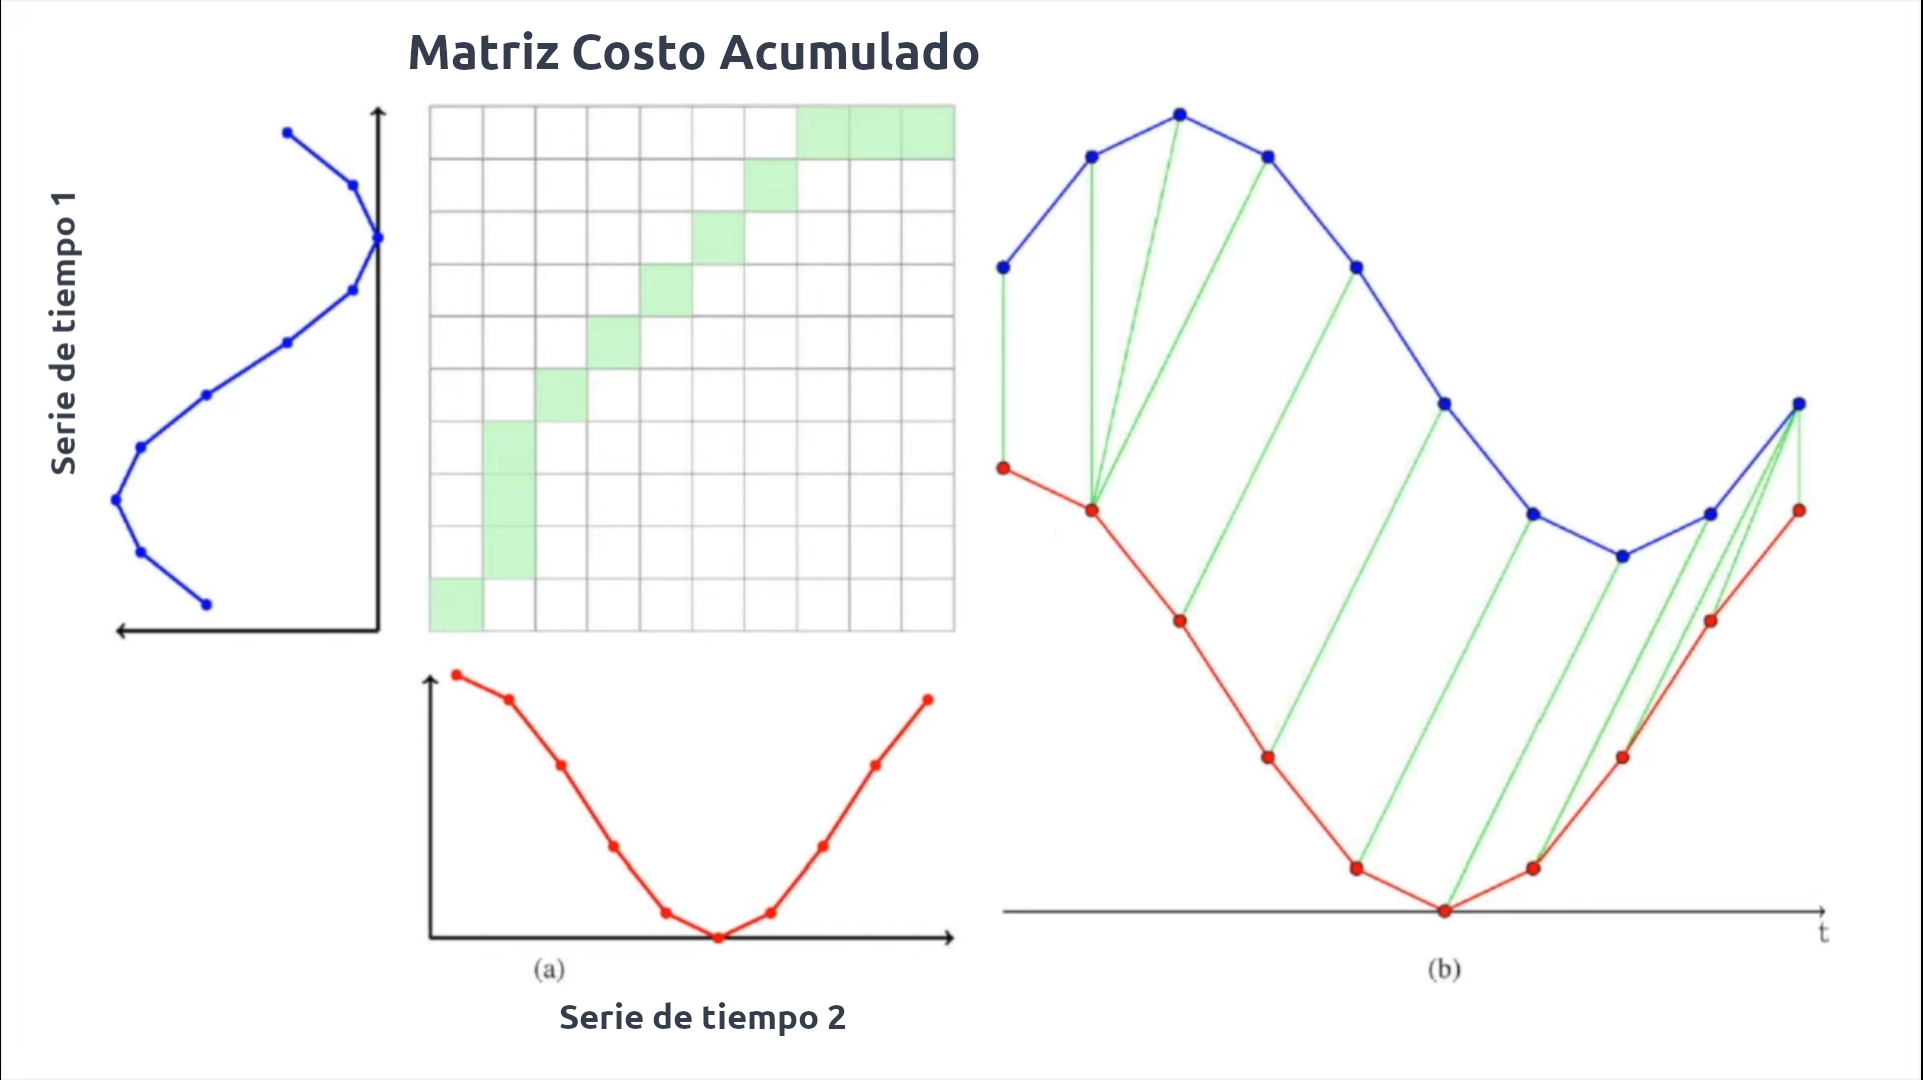
\includegraphics[width=\linewidth]{Imagenes/dtw.png}
		\label{dtw}
		\captionof{figure}{a) Matriz de costo acumulada del cálculo de la distancia entre la Serie de tiempo 1 y Serie de tiempo 2. Los recuadros verdes conforman el camino de deformación óptimo(\textit{optimal warping path}) $p^*$. \\b) Resultado de la alineación óptima para la Serie de tiempo 1 en la Serie de tiempo 2 utilizando DTW. \\{\small Figura recuperada de: Thales Sehn Körting(Productor).(2017) \textit{How DTW (Dynamic Time Warping) algorithm works}[YouTube]. https://www.youtube.com/watch?v=\_K1OsqCicBY}}
	\end{minipage}

\hfill\break
\justifying
\textbf{Banda Sakoe-Chiba}
	\hfill\break
	\justifying
	DTW es un algoritmo muy popular por sus excelentes resultados en la comparación de secuencias temporales, y sin embargo debido a la construcción de la matriz de costos, su complejidad cuadrática es un detractor significativo en tiempo y precisión de cálculo. Una variante común en DTW que aborda esta situación es la implementación de la banda Sakoe-Chiba[15].
	
	\hfill\break
	\justifying
	De forma general, la implementación de restricciones a DTW aporta un par de beneficios. El primero de ellos y el más importante si se plantea el objetivo de la optimización, es la reducción de complejidad con la implementación de la banda, forzando al cálculo de un subconjunto del espacio global e inmediatamente reduciendo su complejidad de $O(L^2)$ a $O(w\times L)$ con $0\geq w \leq L-1$, donde \textit{w} define una banda.
	
	\hfill\break
	\justifying
	El segundo de los beneficios refiere en cuanto a la fiabilidad de la similitud, pues previene alineaciones patológicas, evitando la desviación excesiva de la diagonal principal al camino óptimo posible.
	
	\hfill\break
	\justifying
	La banda Sakoe-Chiba corre a lo largo de la diagonal principal y tiene un ancho fijo $T \in \mathbb{N}$ horizontal y verticalmente(Figura 3). Esta restricción implica que para un elemento $x_n$ puede ser alineado únicamente a uno de los elementos de $y_m$ con $m \in \left[ \frac{M-T}{N-T} \times (n-T), \frac{M-T}{N-T} \times n+T \right] \cap [1:M]$. En la matriz de costo acumulado la ventana de deformación(\textit{warping window} o WW) se observa como en la Figura 3.
	
	\begin{minipage}{\linewidth}
		\centering
		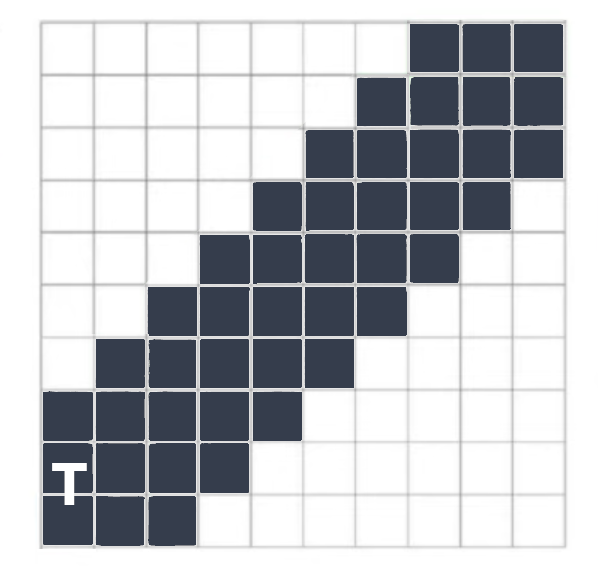
\includegraphics[width=6.5cm]{Imagenes/sakoe-chiba.png}
		\captionof{figure}{Banda de Sakoe-Chiba que corre sobre la diagonal principal de la matriz y que tiene un ancho fijo \textit{T}}
	\end{minipage}

\hfill\break
\justifying
\textbf{Optimización del tamaño de la ventana de DTW}
	\hfill\break
	\justifying
	El algoritmo DTW es un método robusto y con una extraordinaria competitividad, además de utilidad, probando ser una medida de distancia para series de tiempo excepcionalmente fuerte, y sin embargo parte de la comunidad subestima la capacidad del algoritmo por la ignorancia de lo importante que resulta la optimización del tamaño de la ventana \textit{w}, la cual es crítica en la disminución del error durante la predicción[16].
	
	\hfill\break
	\justifying
	Argumentando que la restricción en su cantidad máxima de deformación, cuando es establecida correctamente, cierra la mayoría de los espacios de mejora obtenidos con métodos de clasificación de series de tiempo ''más sofisticados'', el \textit{paper}[17] propone un método novel para el aprendizaje del parámetro óptimo en configuraciones supervisadas y no supervisadas, siendo el caso primero el que compete a este trabajo.
	
	\hfill\break
	\justifying
	Existe una concepción erronea del valor de \textit{w} dependiente del dominio de cálculo por única vez, cuando en realidad no existe un solo valor de \textit{w} que pueda ser transferible entre diferentes contextos, el valor óptimo para la banda restrictiva de DTW dependerá de 2 factores, el número de instancias del conjunto de datos y la estructura propia de los datos, contundentemente abatiendo la posibilidad de la existencia de un valor prototípico de \textit{w} para aplicaciones específicas como ritmos cardiacos o gestos[17].
	
	\hfill\break
	\justifying
	Formalmente el problema se plantea como: Dado un conjunto de entrenamiento de series de tiempo etiquetadas, encontrar el valor de \textit{w} que maximiza la calidad de clasificación en un conjunto de prueba sin etiquetar.
	
	\hfill\break
	\justifying
	La evaluación de la calidad de clasificación se realiza mediante la medida de la precisión.
	
	\hfill\break
	\justifying
	Debido al creciente consenso que ubica al método DTW-k-NN como una línea base robusta, deciden los autores del paper utilizar al algoritmo k-NN como el clasificador subyacente. Como se describe en secciones posteriores, este método es utilizado en todos los modelos evaluados, de forma que el clasificadores como k-NN y SVM son implementados también con diferencia al paper original.
	
	\hfill\break
	\justifying
	El enfoque que toma este método es particularmente útil cuando el conjunto de entrenamiento es limitado, pues implementa una técnica de remuestreo con la creación de datos sintéticos que remplazan al problema de un número de instancias limitadas.
	
	\hfill\break
	\justifying
	El algoritmo consiste en hacer \textit{N} copias del conjunto de entrenamiento original, remplazando para cada copia una fracción de los datos con remplazos sintéticos, para posteriormente realizar validación cruzada con el fin de aprender el porcentaje de error contra la curva de valores de \textit{w}. Se utiliza el valor promedio de todas las iteraciones \textit{N} para la predicción del mejor \textit{w}.
	
	\hfill\break
	\justifying
	De los componentes lógicos que conforman al método, los de mayor interés son el proceso de creación de un nuevo conjunto de datos con una porción sintética, y la función capaz de otorgar una deformación a una secuencia para otorgar un datos sintético.
	
	\hfill\break
	\justifying
	El proceso de creación de un nuevo conjunto de datos con instancias sintéticas inicia por dividir aleatoriamente el \textit{dataset} de datos, cumpliendo con una relación especificada de porcentaje de datos sintéticos sustitutos, permanece la otra partición sin modificación. Posteriormente utilizando k-Fold Cross Validation, se realiza la división en conjunto de entrenamiento y prueba para medir iterativamente la calidad del clasificador. 
	
	\hfill\break
	\justifying
	La función capaz de sintetizar una serie de tiempo inicia con el encogimiento no lineal de la medición real mediante la elimiación aleatoria de un porcentaje definido por el usuario, de los datos que la compone. Seguido a esto, utilizando una función común a bibliotecas de procesamiento de señales, la nueva serie debe remuestrearse a la misma longitud de la secuencia original, agregando antes de este proceso, un acolchado de la señal al repitiendo en los extremos los últimos y primeros 10 valores respectivamente. Finalmente y terminado el remuestreo, se eliminan los valores de acolchado en los extremos y se obtiene una serie sintética de longitud igual a la original.(Figura 4)
	
	\hfill\break
	\justifying
	Esta técnica requiere la configuración de 3 parámetros para su funcionamiento, utilizando como valores constantes para la experimentación los valores propuestos por los mismo autores del \textit{paper}, 20\% de deformación para la creación de datos sintéticos, una relación de 8 a 2 para la creación del nuevo \textit{dataset} con copias sintéticas como número de instancias mayoritarias, y finalmente el para número de iteraciones \textit{N}, mientras mayor sea su valor mejor, considerandose de forma conservativa en 10.  
	
	\begin{minipage}{\linewidth}
		\centering
		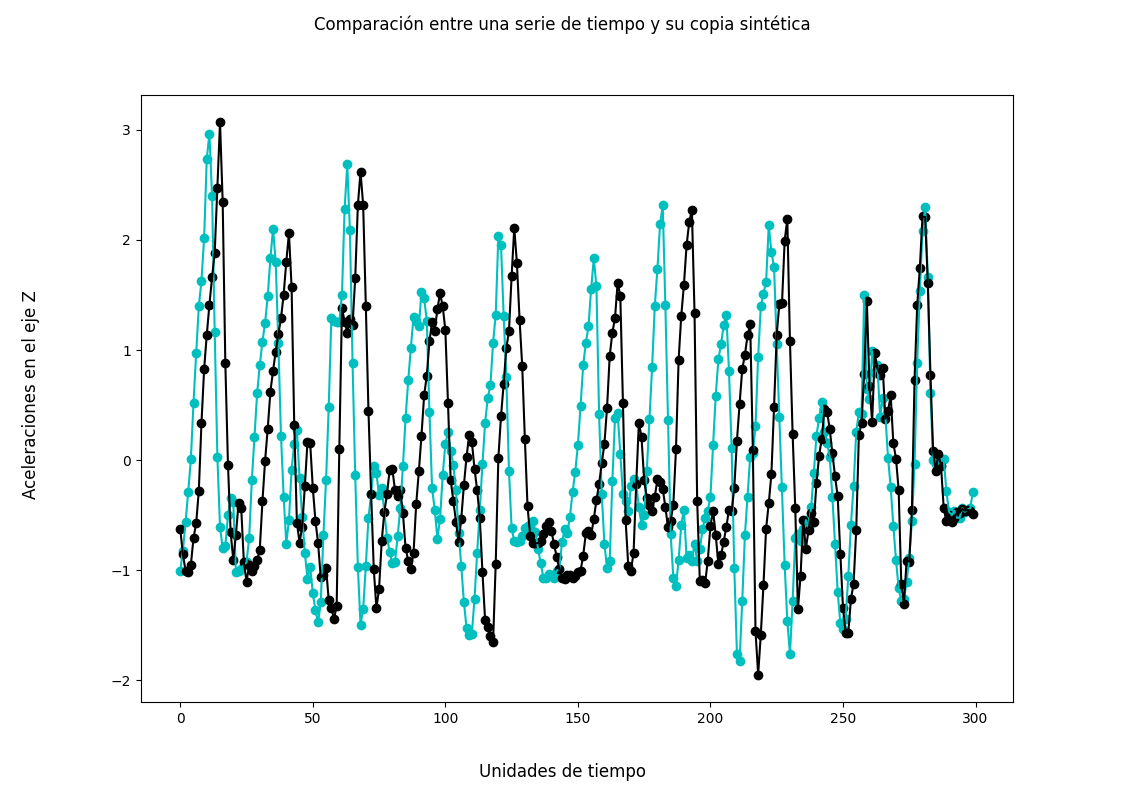
\includegraphics[width=9.5cm]{Imagenes/DTW_sinteticos_2.png}
		\captionof{figure}{Comparación de una instancia perteneciente al \textit{dataset} \textit{GesturePebble}(color azul) y su remplazo sintético(color negro)}
	\end{minipage}
\hfill\break
\justifying
\textbf{PAA}
	\hfill\break
	\justifying
	\textit{Piecewise Aggregate Approximation}(PPA) es un algoritmo que tiene como idea básica la reducción dimensional de una serie de tiempo de entrada mediante la partición de esta en segmentos del mismo tamaño, sobre cada cual se realiza el cálculo promedio de los valores en el segmento[18]. Con una serie de tiempo $Y = Y_1,Y_2,...,Y_n$ con tamaño $n \in \mathbb{R}$ la partición o reducción a una serie $X = X_1,X_2,...,X_m$ donde $m\leq n$, la ecuación que describe los elementos en la serie reducida es:
	
	\begin{equation*}
		\overline{X_i} = \frac{m}{n} \sum_{j=\frac{n}{N(i-1)+1}}^{\frac{n}{M}i}x_j
	\end{equation*}
	
	\hfill\break
	\justifying
	El aspecto más interesante del algoritmo es la forma en que se crean los segmento del mismo tamaño. Es importante notar que antes de realizar la aproximación promedio de cada ventana, el vector debe ser z-normalizado, y una vez haya sido estandarizado el vector la aproximación por partes se calcula.
	
	\hfill\break
	\justifying
	Identificados 2 casos escenciales durante la separación en segmentos. El caso trivial, $m<n$ y \textit{m} es múltiplo de \textit{n}, se trata dividiendo el vector en ventanas de tamaños iguales, sobre las que posteriormente se les realiza un cálculo del promedio para la asignación del nuevo valor a cada segmento. Por otra parte donde $m<n$ y \textit{m} no es múltiplo de \textit{n}, deja de existir un balance que evita la división exacta del vector en segmentos de mismo tamaño. Lo que ahora se requiere es que cada ventana sea redimensionada de forma que cada elemento de la serie de salida es el promedio de un segmento de mismo tamaño al vector de entrada[18].
	
	\hfill\break
	\justifying
	Se observa un ejemplo en la Figura 5 de la discretización de un par de series de tiempo con pocos atributos pero de extensión distinta, que despues de la transformación PAA son equiparables en longitud con un número de palabras \textit{m=9}.
	\begin{minipage}{\linewidth}
		\centering
		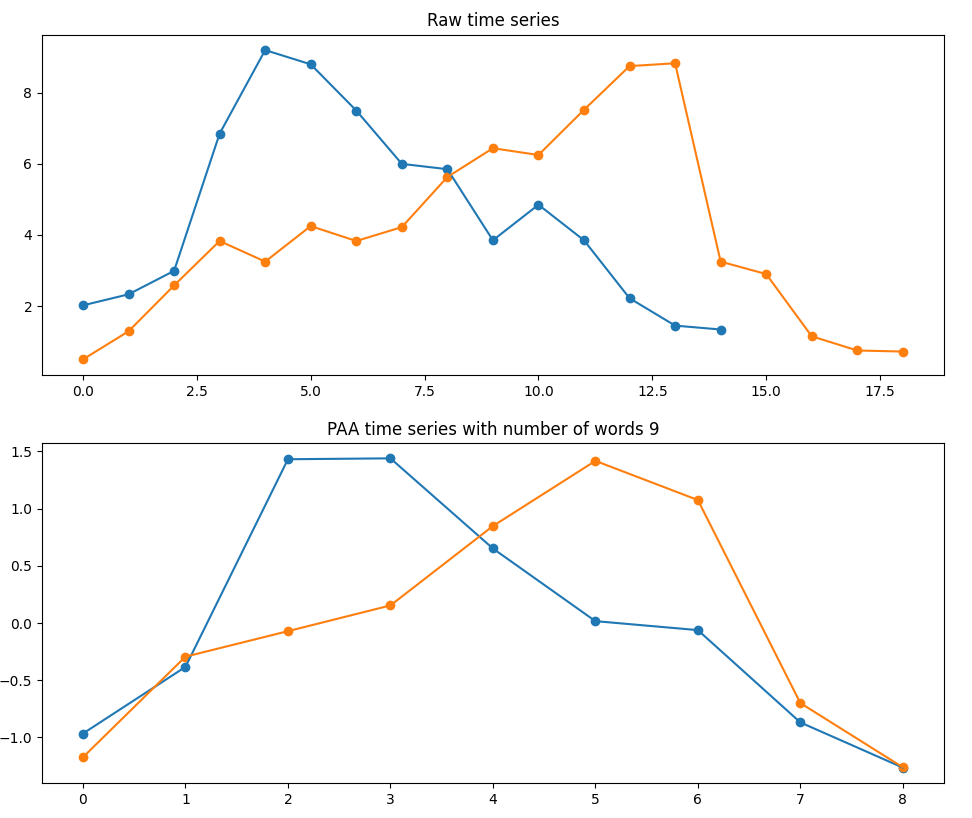
\includegraphics[width=\linewidth]{Imagenes/PAA.png}
		\captionof{figure}{Con el algoritmo PAA se mantienen las tendencias de las secuencias temporales, con la diferencia que han sido reducidos el número de valores que las conforman, nombradas palabras después de la discretización.}
	\end{minipage}
	
\hfill\break
\hfill\break
\justifying
\textbf{Symbolic Aggregate Approximation}
	\hfill\break
	\justifying
	SAX es una técnica desarrollada y enfocada en la reducción dimensional de una serie numérica con una serie de tiempo, a un espacio simbólico de 'palabras'. Dada una serie dependiente del tiempo de longitud arbitraria \textit{n} se realiza la transformación a una cadena de longitud \textit{w} utilizando un alfabeto $A={a_1,a_2,...,a_3}$[19].
	
	\hfill\break
	\justifying
	La primer parte de la discretización es manejada por la transformación PAA. siguiendole entoces el proceso de asignación de símbolos para cada sección, siendo requerimiento para esta segunda parte de la discretización, que los símbolos sean asignados equiprobablemente(propiedad de una colección de eventos teniendo la misma probabilidad de ocurrir). Esto se cumple facilmente por la previa normalización de los datos de la serie en una distribución Gausiana, por lo que las áreas bajo la curva de campana de la distribución pueden ser utilizadas para la creación de los puntos de quiebre(\textit{breakpoints}) en los datos normalizados para la asignación de palabras.
	
	\hfill\break
	\justifying
	El proceso del algoritmo toma los siguientes procesos en el siguiente orden[13]:
	\begin{enumerate}
		\item Estandarización o normalización-z de los datos de la serie de tiempo para tener una media de 0 y una desviación estándar de 1
		\item Transformación o reducción de dimensionalidad desde \textit{n} a \textit{w} mediante el algoritmo \textit{Piecewise Aggregation Approximation}(PAA)
		\item Asignación de los puntos de quiebre $\beta = \beta_1,...,\beta_{\alpha-1}$
		\item La serie de tiempo es discretizada tomando el promedio de cada segmento para ser mapeado a un alfabeto \textit{A}
	\end{enumerate}
	
	\hfill\break
	\justifying
	La distancia entre 2 Palabras o cadenas, correspondiendo cada una a diferentes series de tiempo, se calcula como el promedio de los pares de las distancias de símbolos.
	
	\hfill \break
	\textbf{Puntos de quiebre}
	\justifying
	Los puntos de quiebre es una lista de números $\beta = \beta_1,...,\beta_{\alpha - 1}$ tal que el área debajo la curva gausiana de $\beta_i$ a $\beta_{i+1}=\frac{1}{\alpha}$[19].
	
	\hfill\break
	\justifying
	Estos puntos de quiebre pueden ser obtenidos mirando una tabla estadística y puede ser utilizada para discretización de series de tiempo donde el coeficientes debajo el punto de quiebre más pequeño son mapeados a la letra del alfabeto en el índice 1, mientras los coeficientes mayores o igual al punto de quiebre más pequeño y menor al segundo punto de quiebre se le asigna la letra del alfabeto con el segundo ínidice, y así se sigue.
	
	\hfill \break
	\textbf{Distancia SAX}
	\justifying
	La distancia entre 2 símbolos se define a 0 si el índice difiere a lo más por 1(por ejemplo resulta 0 entre símbolos $a_i$ y $a_{i+1}$), en cualquier otro caso la distancia entre símbolos $a_i$ y $a_k$, donde $k>i$, se define como $b_{k-1}-b_i$[13].
	
	\hfill\break
	\justifying
	La distancia entre 2 cadenas correspondientes a diferentes series de tiempo, se calcula como el promedio de las distancias de los símbolos por parejas(por ejemplo; el promedio de la distancia entre el primer símbolo de cada serie, la distancia entre el segundo símbolo de cada serie, y así sucesivamente)[13].

\end{multicols}

\begin{figure}[!h]%
\begin{center}%
	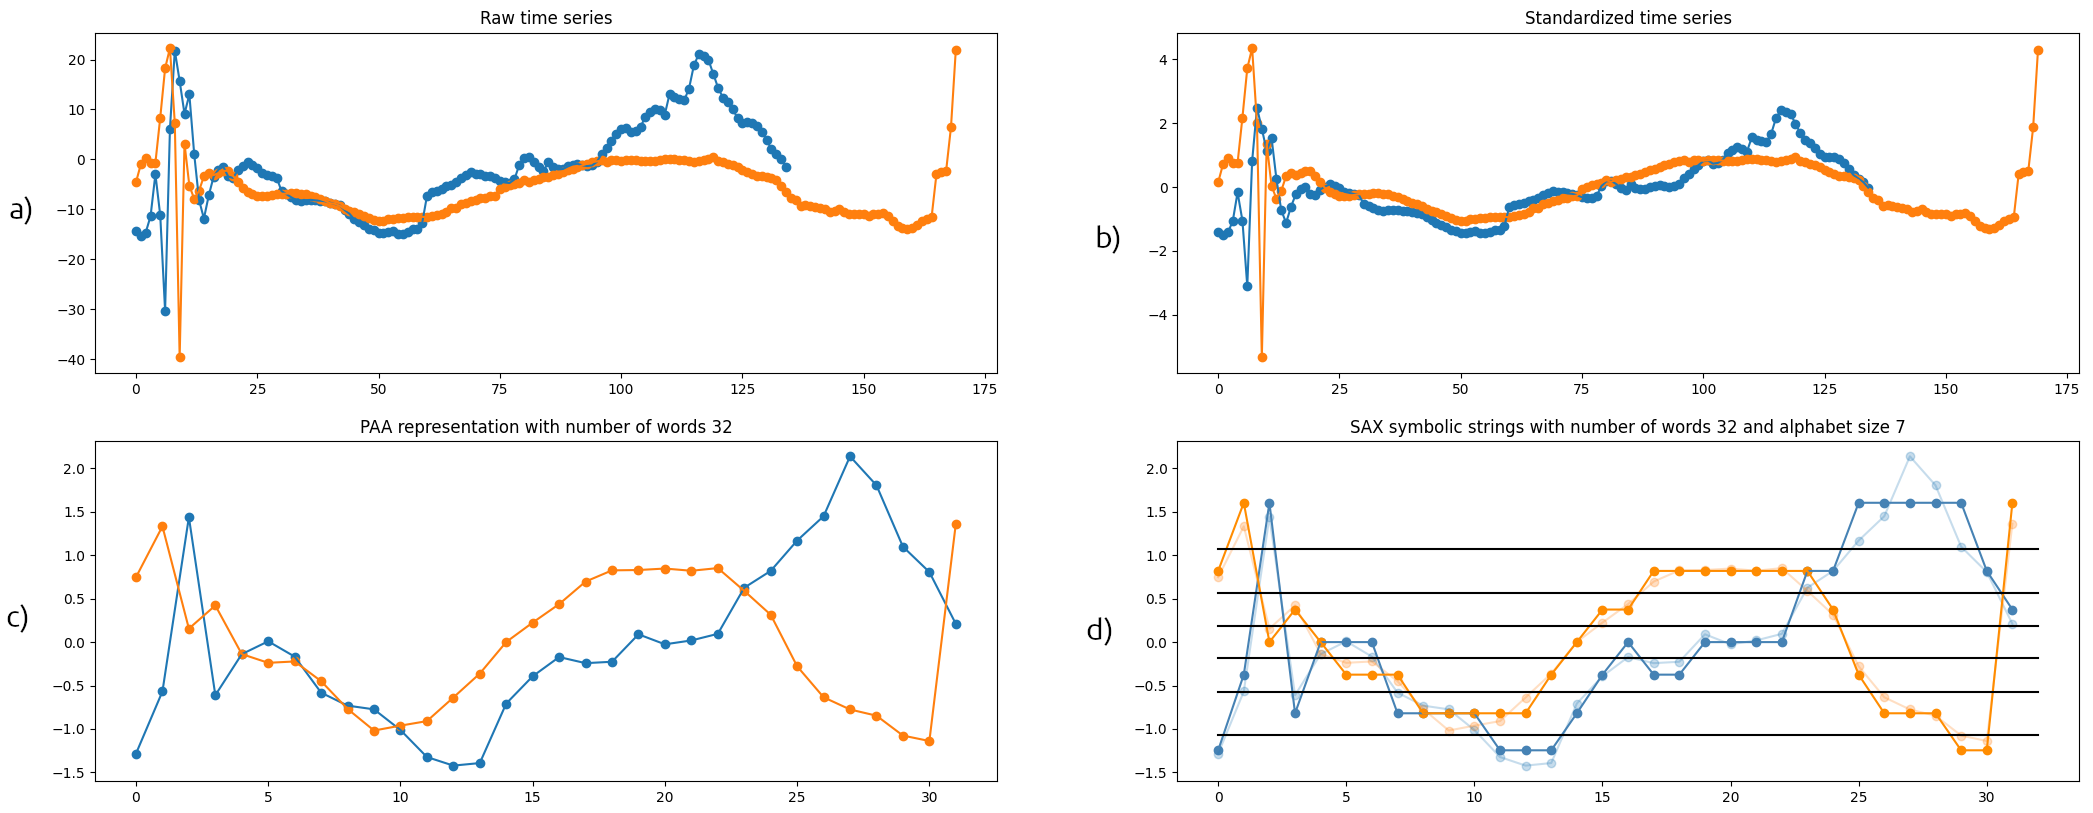
\includegraphics[width=\columnwidth]{Imagenes/SAX_example_2.png}%
	\caption{Graficación de un par de series de tiempo tomadas del \textit{dataset} \textit{GesturePebble} durante el proceso completo de la discretización SAX\\a) Series de tiempo de longitud variables con valores reales(originales)\\b) Series de tiempo después de estandarización.\\c) Series de tiempo después de la transformación PAA con un número de palabras igual a 32.\\d) Series de tiempo en su representación SAX como una cadena de símbolos numéricos con alfabeto de tamaño 7(En el fondo difuminadas se encuentra como referencia las mismas secuencias en representación PAA previo la discretización en símbolos de la cadena SAX).}
	\label{label}%
\end{center}%
\end{figure}%

\begin{multicols}{2}
\hfill\break
\justifying
\textbf{DTW Barycenter Averaging}
	\hfill\break
	\justifying
	\textit{DTW Barycenter Averaging}(DBA) es un algoritmo iterativo que utiliza DTW para la alineación de series de tiempo a ser promediadas con un promedio envolvente[20]. Introducido por Petitjean, la implementación del algoritmo DBA trae consigo varias ventajas importantes frente a un proceso plano o simple de promediación de un conjunto de secuencias.
	
	\hfill\break
	\justifying
	El algoritmo \textit{grosso modo}, opera de la siguiente manera:
	\begin{enumerate}
		\item Las \textit{n} series por ser promediadas son etiquetadas $S_1,S_2,...,S_n$ y tienen una longitud \textit{T}.
		\item Se inicia el proceso con una serie abreviada inicial \textit{A}.
		\item Mientras el promedio no haya convergido:
			\begin{enumerate}
				\item Por cada serie \textit{S}, se aplica DTW contra \textit{A} y se salva el camino de deformación.
				\item Se utiliza el camino de deformación y se construye un nuevo promedio de \textit{A} al dar a cada punto un nuevo valor: El promedio de cada punto de \textit{S} conectado a este en el camino de deformación resultante de DTW.
			\end{enumerate}
	\end{enumerate}

	\hfill\break
	\justifying
	Una buena inicialización del proceso con un candidato correcto para \textit{A}, es de extrema importancia, porque mientras el proceso DBA por si mismo es determinístico, el resultado final dependerá escencialmente on la secuencia abreviada inicial. Se identifican entonces 3 objetivos distintivos:
	\begin{itemize}
		\item Preservar la forma de las entradas.
		\item Preservar la magnitud de los extremos en el eje y.
		\item Preservar la sincronización de aquellos extremos en el eje x.
	\end{itemize}

	\hfill\break
	\justifying
	En el \textit{paper} se recomienda inicializar DBA eligiendo de forma aleatoria la serie abreviada de inicio \textit{A}, y en un principio esta técnica preserva bien la forma, pero la sincronización de los extremos dependerá en cual serie resulta escogida, razón por la que un proceso deterministico de elección es preferible.
	
	\hfill\break
	\justifying
	Una solución consiste en utilizar una serie de entrada para la inicialización, escogiendo mediante un proceso determinístico la entrada. Como primer paso de debe elimina la tendencia de cada una de las instancias en la serie, para paso seguido, guardar el valor en el eje x de los valores máximos y mínimos de cada serie. Finalmente la serie de inicialización abreviada, será la más cercana a la media de los valores guardados. Este proceso conserva la forma de las secuencias, las magnitudes extremas en el eje de las ordenadas, y finalmente obtener una noción clara de las posiciones típicas para x de aquellos extremos.
	
\end{multicols}

\hfill\break
\begin{figure}[!h]%
	\begin{center}%
		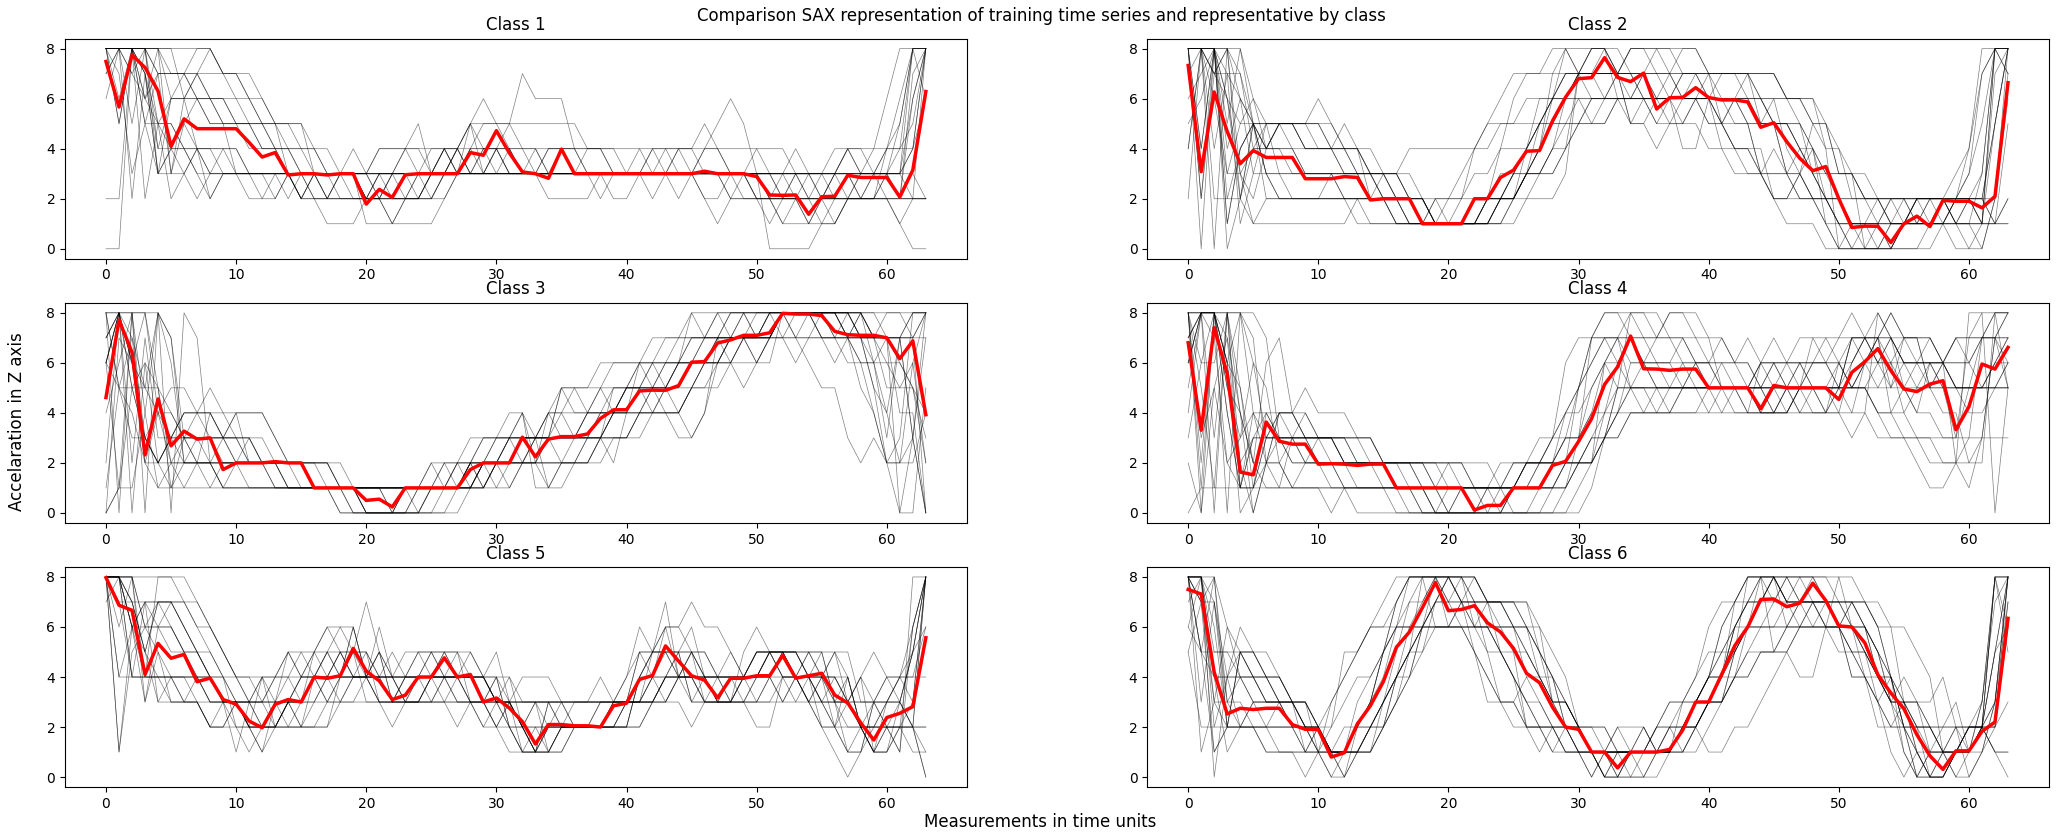
\includegraphics[width=\columnwidth]{Imagenes/DBA.png}%
		\caption{Ejemplo de las series representantes de cada clase para el conjunto de datos \textit{GesturePebble}. Cada representante(color rojo) fue calculada utilizando el algoritmo DBA con un promediado de 5 instancias discretizadas(color negro) en representación SAX de alfabeto tamaño 9 y número de palabras 64.}
	\end{center}%
\end{figure}%

\begin{multicols}{2}
		
		\hfill\break
		\centering
		V. ~~~~~~ MÉTODOS DE CLASIFICACIÓN
		
		\hfill\break
\justifying
\textbf{DTW 1-NN}
	\hfill\break
	\justifying
	Un modelo obligatorio como punto de partirda entre las bastas alternativas de técnicas que atienden el problema TSC, es a través de una combinación del algoritmo DTW y el modelo \textit{k-NN}, para la clasificación de sequencias dependientes del tiempo, mostrando sus capacidades de precisión y robustez cuando comparado con técnicas más poderosas[21].
	
	\hfill\break
	\justifying
	Esta robusta técnica combina la medida de similitud entre secuencias de tiempo DTW y el algoritmo de clasificación k-NN(\textit{k Nearest Neighbours}) en su variante con \textit{k=1}, parámetro definido de forma empírica por inifindad de trabajos anteriores y para conformar actualmente el método base en el problema de TSC por la creciente aceptación por parte de la comunidad.
	
	\hfill\break
	\justifying
	En esta variante del algoritmo k-NN, se sustituye la distancia Euclideana como función de medida entre los datos, por la medida de similitud DTW entre series de tiempo, resultando en su gran capacidad de clasificación con una buena precisión. Aún con los beneficios que otorga el modelo referencia, es importante revisar los detrimentos de la técnica frente a las limitaciones y condicionantes naturales de la problemática que se atiende. La gran debilidad de este algoritmo reside en la complejidad y tiempo de cálculo, dado principalmente por el uso de función de medida a DTW en el modelo clasificador.
	
	\hfill\break
	\justifying
	La complejidad cuadrática de DTW, $O(N^2)$, cuando se evalua la similitud de la series de tiempo que se intenta predecir con respecto al número de instancias que conforman el conjunto de datos de ''entrenamiento'', incrementa significativamente el número de cálculos derivado de la conformación de la matriz de costo del algoritmo. Frente a esta situación, se ha buscado la optimización del algoritmo utilizando las restricciones, en un intento de disminuir la complejidad en la conformación de la matriz de costo acumulada, inevitablemente requiriendo el aprendizaje del tamaño óptimo del parametro \textit{w}, restringiendo los cálculos a elementos más cercanos a la diagonal.
	
	\hfill\break
	\justifying
	La versión desarrollda experimentalmente en este trabajo, implementa la técnica de optimización del tamaño de la ventana DTW[17], en la búsqueda de satisfacer las condiciones de la solución que exígen un modelo optimizado sin dejar de lado una buena precisión en la predicción.
	
\hfill\break
\justifying
\textbf{Modelo SAX-DTW}
	\hfill\break
	\justifying
	Técnica propuesta en el paper \textit{''Gesture recognition using Symbolic Aggregate Approximation and Dynamic Time Warping on motion data''}[13], como el método mas preciso de entre los 3 evaluados, y que supera a los demás al reportar una razón promedio de clasificación correcta igual al 99.21\%.
	
	\hfill\break
	\justifying
	El método se basa en la coexistencia del algoritmo SAX y la función de medida DTW, logrando combinar las mejores características de ambos métodos; La efectividad y baja complejidad de SAX, con la insensibilidad de DTW a las fluctuaciones de velocidad durante la ejecución de un gesto[13].
	
	\hfill\break
	\justifying
	Este segundo método, al igual que el de referencia, utiliza como clasificador subyacente a 1-NN, pero implementado como función de distancia, la propia distancia SAX modificada para implementar la alineación óptima de DTW.
	
	\hfill\break
	\justifying
	La totalidad de las secuencias temporales serán discretizadas a la representación SAX, tanto las instancias de conjunto de ''entrenamiento'', como los nuevos patrones ingresados para su etiquetado mediante predicción.
	
	\hfill\break
	\justifying
	Importante para el método SAX aclarar los valores de los parámetros utilizados. En el \textit{paper} desarrollan sus experimentos con un valor para el número de palabras igual a 32(Representación PAA), y un tamaño de alfabeto igual a 7.
	
	\hfill\break
	\justifying
	Finalmente la funcion de medida adopta el concepto de la distancia entre 2 símbolos SAX, con un modificación que ocupa el camino óptimo de deformación, proponiendo una comparación de la distancia entre símbolos relacionados por el camino DTW en vez de la comparación por defecto entre los pares de símbolos, y que elige al par que corresponde al símbolo de cada una de las cadenas en el mismo índice(una comparación de distancia Euclideana en el ámbito discreto simbólico de SAX). En la Figura 8 se ilustra el uso del método SAX-DTW.
	
	\hfill\break
	\justifying
	La implementación del algoritmo DTW en este método exige la optimización del parámetro \textit{w}, como restricción en forma de banda Sakoe-Chiba, aplicándose también durante los resultados de la experimentación, el método de aprendizaje del tamaño óptimo de ventana[17].
	
	\begin{minipage}{\linewidth}
		\centering
		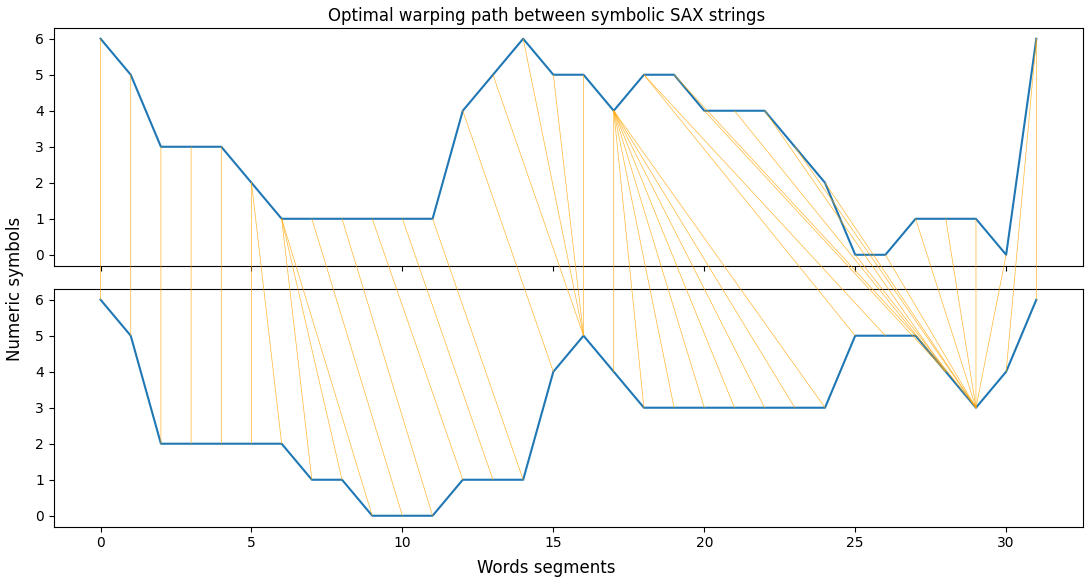
\includegraphics[width=\linewidth]{Imagenes/SAX_DTW.png}
		\captionof{figure}{Algoritmo del camino de deformación óptima calculada por DTW sobre 2 cadenas simbólicas SAX.}
	\end{minipage}
	
\hfill\break
\justifying
\textbf{Método vectores de atributos distancia DTW de series de tiempo SAX}
	\hfill\break
	\justifying
	Como método original propuesto en este trabajo, se busca al igual que el segundo método, la coexistencia y adición de los beneficios que ofrece la disminución dimensional y discretización por parte de las representaciones SAX, con la robustez en el proceso de medición de la similitud de DTW para series con extensión y velocidades distintas. Aún cuando ambos algoritmos se implementan en un mismo modelo, el enfoque y filosofía de funcionamiento del modelo difiere del segundo, implementado una técnica desarrollada en el \textit{paper}[22] y que propone representar a una serie de tiempo en conformando los atributos de distancias DTW en comparación de cada ejemplo de entrenamiento[22].
	
	\hfill\break
	\justifying
	Así como el método toma inspiración de las técnicas desarrolladas en ambos artículos[17,22], ninguna de las técnicas se aplica fielmente tal y como los describen los autores en sus respectivos trabajos.
	
	\hfill\break
	\justifying
	Un cambio especialmente importante en comparación a los métodos descritos anteriormente, es la implementación de un algoritmo \textit{Machine Learning} mucho más robusto al sencillo k-NN. ocupándose un clasificador de soporte vectorial, y que forma parte de las ventajas y posibilidades de mejora al conformarse vectores de atributos distancia DTW[22].
	
	\hfill\break
	\justifying
	Apalancándose del hecho de que la manera más sencilla de obtener una mejora en la precisión de la clasificación para secuencias dependientes del tiempo, es la implementación de un método basado en características(Representación estadística o simbólica definida para una serie de tiempo), se requiere la transformación de los datos en un espacio alternativo donde las características discriminatorias pueden ser más facilmente detectables que un clasificador más complejos en el tiempo[6]. 
	
	\hfill\break
	\justifying
	El manejo de la totalidad de series de tiempo se realiza mediante las cadenas simbólicas resultantes del algoritmo SAX, que proveé además de una transformación a un espacio alternativo de dominio simbólico, una reducción dimensional, lo que traduce en una simplificación de la complejidad. Esto implica que ninguna de las etapas siguientes pueda realizarse sin antes transformar las secuencias en cadenas simbólicas con número de palabras iguales a 64 y su discretización en el dominio de valores con un alfabeto tamaño 9.
	
	\hfill\break
	\justifying
	Pensando en aprovechar todo el potencial de las similitudes calculadas por DTW, se escoge un alfabeto numérico en las representaciones SAX, con la finalidad de utilizar sin realizar una previa modificación de los símbolos la distancia DTW. Este alfabeto numérico de tamaño 9, ofrece los dígitos enteros dentro el rango $[0,8]$ como el conjunto de símbolos que conformand las cadenas SAX.
	
	\hfill\break
	\textbf{Proceso de entrenamiento}
	\justifying
	Cuando se involucra un método de \textit{Machine Learning} como SVC, el modelo debe pasar por una etapa de entrenamiento antes de poder ofrecer la tarea de predicción, situación que no sucede con el algoritmo k-NN de los métodos previos, pues realmente la etapa de entrenamiento y predicción sucede en un proceso integral.
	
	\hfill\break
	\justifying
	La creación de los vectores de atributos en este método es escencial, no solo por la posibilidad que ofrece de aplicarse como entrada a modelos robustos de \textit{Machine Learning}, pero por que además diverge del paper[22] en el que se inspira, y se toma una interpretación alternativa que impacta positivamente las etapa de entrenamiento y predicción, pero siendo de mayor relavancia su ventaja durante la predicción; Disminuyendo significativamente el tiempo de cálculo y complejidad requerido para la creación del vector de instancias por cada secuencia temporal.
	
	\hfill\break
	\justifying
	Tomando un enfoque alternativo a la creación del vector de atributos, antes de pasar si quiera a esta etapa, se requiere crear una cadena simbólica representante de cada clase existente en el conjunto de datos, y como requsito se exige la estratificación del conjunto para mantener la equiprobabilidad de las clases durante el entrenamiento.
	
	\hfill\break
	\justifying
	La fabricación del conjunto de cadenas representantes se logra mediante el promediado de
	todos los vectores existentes en el conjunto de datos que pertenecen a una misma clase, y el método más efectivo para lograr un representante fidedigno de cada etiqueta es DBA[20].
	
	\hfill\break
	\justifying
	Este conjunto de representantes resultante se convierte a partir de su cálculo, en el conjunto de cadenas simbólicas más importantes del modelo. El hecho de que mediante la similitud DTW de estos representantes con los vectores destinados al entrenamiento y posteriormente los nuevos patrones a ser predecidos, exige la preservación del conjunto durante la vida útil del modelo entrenado. A pesar de tratarse de un algoritmo determinístico que sugiere el recálculo del conjunto de representantes frente a la pérdida de este, si la elección de la serie de tiempo abreviada inicial \textit{A} se obtiene por un proceso aleatorio, el cálculo una segunda vez del conjunto de representantes significaría desechar el modelo entrenado para volver a crear las instancias de entrenamiento con este nuevo conjunto.
	
	\hfill\break
	\justifying
	Creado el conjunto de cadenas representantes de cada clase, se calculan los vectores de atributos distancia DTW entre la instancia de entrenamiento y los representantes de clase(es importante el orden en que se ingresan ambas cadenas simbólicas, pues la operación de similitud DTW no es conmutativa), ingresándolos en el modelo SCV para iniciar la etapa de entrenamiento.
	
	\hfill\break
	\textbf{Proceso de predicción}
	\justifying
	Muestreado, filtrado y preprocesado un patrón de movimiento, el primer paso será representarlo mediante SAX en una cadena simbólica con un alfabeto numérico.
	
	\hfill\break
	\justifying
	Como cadena simbólica, ahora esta secuencia puede ser usada para conformar un vector de atributos distancia DTW utlizando el mismo conjunto de representantes de clase usado para fabricar los vectores de entrenamiento.
	
	\hfill\break
	\justifying
	Finalmente el vector resultante puede ser alimentado al modelo SVC previamente entrenado para la obtención de la etiqueta de clase resultante del proceso de predicción.
		
		\hfill\break
		\justifying
		
		\hfill\break
		\centering
		VI. ~~~~~~ RESULTADOS EXPERIMENTALES
		
		\hfill\break
\justifying
El proceso experimental consiste en la replicación de los modelos descritos teóricamente en la sección previa, aplicando inicialmente el método de optimización para el tamaño de la ventana \textit{w} para cada uno de los modelos, y posteriormente midiendo la precisión del modelo utilizando el óptimo valor de \textit{w} para el entrenamiento y fase de predicción con el \textit{dataset} completo \textit{GesturePebbleZ1}.

\hfill\break
\justifying
Se decidió por Python como el lenguaje de programación utilizado para la implementación y prueba de los modelos, parte por la gran disponibilidad de bibliotecas relacionadas con modelos de \textit{Machine Learning} y especializadas en la Clasificación de Series de Tiempo, aunque estos tan solo se tomaron como referencia pues la mayoría se desarrolló igualmente.

\hfill\break
\justifying
Todos los algoritmo y técnicas utilizadas fueron desarrolladas en módulos de uso particular para la replicación de los modelos en este trabajo, con excepción de la función DBA, la cual si forma parte de la biblioteca nombrada \textit{tslearn} y no se desarrollo directamente. Igualmente a lo que refiere a los modelos clasificadores de machine learning, se implementaron funciones parte de las bibliotecas desarrolladas, encargadas de ejecutar el sencillo algoritmo 1-NN con las variaciones necesarias para la adición de las diferentes funciones de medición con el modelo referencia y el modelo propuesto en el trabajo de reconocimiento de gestos utilizando dispositivos comúnes[13]. La excepción se encuentra en el algoritmo SVC, para el cual se utilizó la función que ofrece scikit-learn, requiriendo únicamente el ingreso de los conjuntos de entrenamiento, conjunto de clases y especificación de parámetros en la fase de entrenamiento, y el vector por predecir para la fase de clasificación.

\hfill\break
\justifying
Se puede visitar el GitHub del proyecto donde se encuentran los archivos de la implementación por modelo, programas de prueba para cada una de las técnicas y funciones desarrolladas, el par de bibliotecas con las técnicas y algoritmos(\textit{Libraries} y \textit{LLibraries}), una carpeta con los \textit{dataset} utilizados y finalmente una carpeta de resultados con los datos obtenidos por cada modelo: {\small \underline{https://github.com/LaloValle/Clasificador\_vector\_atributos\_SAX-DTW}} .

\hfill\break
\justifying
La implementación del algoritmo DTW en los 3 modelos requirió el aprendizaje del valor óptimo de la ventana para cada uno de los modelos[13], pues como se ha explicado previamente, no existe valor único de \textit{w} que pueda ser intercambiable entre contextos, la forma de los datos y el tamaño del conjunto, son factores que afectan a la universalidad de este valor, y como se explica, el manejo de los datos como la etapa en la que DTW interviene, suele ser distinto para cada modelo.

\hfill\break
\justifying
Para ejecutar la técnica de optimización del parámetro \textit{w}, se utilizó el \textit{dataset} \textit{GesturePebbleZ1\_TRAIN}, que consta de un total de 132 entradas considerando un total de 6 etiquetas de clase distintas. La técnica de optimización que se implementa requiere de un modelo estratificado, de forma que después de la estratificación el conjunto de entrenamiento cuenta con un total de 120 entradas, 20 secuencias temporales por cada clase. Los demás parámetros que se consideran comúnes para todos los modelos son el número de iteraciones \textit{N} igual a 10 y \textit{k-Fold Cross Validation} igual a 10.

\hfill\break
\justifying
Los límites inferiores y superiores del cálculo de \textit{w}, si cambian en función del modelo y se definieron despues de realizarse una iteración de prueba con un limite superior relativamente alto para identificar el rango de valores donde el modelo aumenta su precisión y para evitar calcular todos los posibles valores de \textit{w}(455,32 y 64 respectivamente para cada modelo) junto con un 10-FCV, repitiendo 10 iteraciones para cada valor de ventana. Los rangos por modelo quedaron de la siguiente forma:
\begin{itemize}
	\item DTW 1-NN: $[11,17]$
	\item SAX-DTW[13]: $[2,8]$
	\item Atributos SAX-DTW(Propuesto): $[2,10]$
\end{itemize}

\begin{center}
	\begin{tabular}{c|c c c}
		\multicolumn{4}{c}{Optimización del tamaño de ventana \textit{w}} \\ \hline
		Métodos & Precisión & Tiempo(min) & Valor \textit{w} \\ \hline
		DTW 1-NN &  85.83\% & 25.28 & \textbf{16} \\
		SAX-DTW & 89.83\% & 6.28 & \textbf{2} \\
		Atributos SAX-DTW & \textbf{95.25}\% & 43.45 & \textbf{4} \\
	\end{tabular}
	\captionof{table}{Tabla que muestra los resultados obtenidos para cada método con la técnica de optimización del tamaño de ventana \textit{w}.}
	\label{tabla_optimizacion_w}
\end{center}

\hfill\break
\justifying
En el Cuadro 1 se reportan los resultados obtenidos de la técnica de optimización del valor de la ventana \textit{w}, siendo importante rescatar el reducido tamaño de ventana para el par de métodos que implementan una transformación de espacio a un dominio simbólico mediante SAX, pues la sola traducción de esta valor de ventana en número de operaciones, representa una optimización significativa, pero esto tan solo si no se considera la longitud de las secuencias a las que se les aplica DTW para cada método, pues el uso directo de series de tiempo con 455 valores en longitud, ya es demasiado malo en términos de complejidad para además manejar valores grandes de \textit{w}. Sin embargo dentro su contexto, siempre la optimización del valor del tamaño de ventana, incluso para el método referencia, ofrecerá grandes beneficios a su aplicación sin un \textit{w} correcto.

\hfill\break
\justifying
Calculado el parámetro de ventana del algoritmo DTW, los modelos se encuentran en condiciones de realizar la prueba final de precisión en la predicción utilizando ambos \textit{dataset}, \textit{GesturePebbleZ1\_TRAIN} y \textit{GesturePebbleZ1\_TEST} para sus respectivos contextos. Los datos que se reportan se realizaron fijando los parámetros como se muestra a continuación:

\begin{center}
	\begin{tabular}{c c}
		\textbf{Parámetros} & \textbf{Valores} \\\hline
		Tamaño \textit{dataset} entrenamiento & 120 \\
		Tamaño \textit{dataset} prueba & 150 \\
		Número de corridas & 10 \\
		Tamaño de ventana \textit{w} & Aprendido para cada método \\
		
	\end{tabular}
\end{center}


\begin{center}
	\begin{tabular}{c|c c}
		\multicolumn{3}{c}{Precisión en la predicción} \\ \hline
		Métodos & Precisión & Tiempo(seg) \\ \hline
		DTW 1-NN &  75.20\% & 57.91 \\
		SAX-DTW & 90.33\% & 12.89  \\
		Atributos SAX-DTW & \textbf{94.06}\% & \textbf{5.181} \\
	\end{tabular}
	\captionof{table}{Tabla que muestra los resultados promedio obtenidos en la precisión de la predicción para cada método.}
	\label{tabla_precisión}
\end{center}

\hfill\break
\justifying
Después de la evaluación final en la que se midió la precisión de los 3 modelos al momento de realizar predicciones, se observa claramente el éxito de los modelos basados en características, destacando el desempeño del modelo propuesto en este trabajo por las mejoras muy superior en la precisión frente al modelo referencial, pero presentando también una diferencia pequeña sin embargo significativa de 4 puntos porcentuales a favor, cuando se compara a la técnica de Mezari y Maglogiannis[13].

\hfill\break
\justifying
La optimización durante la etapa de entrenamiento y predicción, es definitivamente el ámbito donde nuestra propuesta de atributos SAX-DTW, lidera y con excelente ventaja, las marcas de tiempo registradas para la predicción de 150 instancias, superando hasta por el doble de rapidez, al segundo método mejor clasificado.
		
		\hfill\break
		\justifying
		
		\hfill\break
		\centering
		VII. ~~~~~~ CONCLUSIÓN Y TRABAJO FUTURO
		
		\hfill\break
\justifying
Analizando los resultados se razona la efectividad y utilidad que cumple la implementación del algoritmo de transformación espacial SAX, resaltando el efecto que tiene sobre la complejidad, la cual sufre una disminución impresionante en comparación al método referencia, a tal punto que los valores para \textit{w} del algoritmo DTW, se mantienen debajo de 5. El constraste de complejidad, se vuelve evidente con el valor de 16 que optimiza el método para el modelo referencia, técnica que no considera en su algoritmo, tratamiento alguno de las series de tiempo que maneja, aportando además al número de cálculos con el valor 16 de \textit{w}, el hecho de que las secuencias con las que se realiza la función de similitud, son de hasta longitud 455, situación irreverente frente a las longitudeds máximas constantes de 32 y 64 para los ultimos 2 modelos implementados.

\hfill\break
\justifying
El par de métodos basados en características, encabezado por el algoritmo SAX, se les observa no solo disminuye la complejidad y propicia por lo tanto al tiempo de cálculo, factor importante para las condiciones de la solución que se trabaja; Además, ofrece un aumento en la precisión comparando con el método de refencia que se clasifica como un método basado en distancias, factores que terminan por descartar completamente al de referencia como una técnica viable para el problema de la clasificación de gestos motrices.

\hfill\break
\justifying
Durante el análisis de las cifras arrojadas, se notó una discrepancia entre la precisión promedio obtenida en el proceso de aprendizaje del valor óptimo para la ventana \textit{w}, con respecto a la precisión final alcanzada de la evaluación de las predicciones con el conjunto de datos completo \textit{GesturePebbleZ1}. Surgen un par de hipótesis que se consideran en trabajo a futuro como una aclaración de estas diferencias.

\hfill\break
\justifying
La primer hipótesis considera que la diferencia entre las cifras se debe a la naturaleza del \textit{dataset}. Para el entrenamiento y aprendizaje del parámetro \textit{w}(que involucra la evaluación de predicciones) se utiliza el archivo de entrenamiento exclusivamente, donde la naturaleza de su construcción fue con patrones desarrollados por los participantes en el lapso de un mismo día durante la sesión 1. Por su parte la evaluación con el archivo de pruebas del mismo \textit{dataset}, se aclara haber sido realizado en una sesión diferente con días de diferencias. En este caso se induce el origen de la diferencia de las mediciones entre la primer sesión(conjunto de entrenamiento) y la segunda(conjunto de pruebas).

\hfill\break
\justifying
La segunda hipótesis, capaz de ser comprobada y negar o afirmar la primera planteada, deriva del hecho de que durante el proceso de aprendizaje de \textit{w}, se generan nuevas instancias sintéticas que pudieran tener mucho mayor influencia de la considerada en la variabilidad de los casos de entrenamiento, estimulando una clasificación más general y precisa que resulta en una influencia positiva al modelo. Si este fuera el caso, basta con introducir a la prueba final la técnica de fabricación de conjuntos de entrenamiento con datos nuevos dado por un porcentaje de instancias sintéticas, y evaluando la precisión de predicción, seríamos capaces de identificar la más probable naturaleza del déficit localizado entre porcentajes.

\hfill\break
\justifying
Aún con esta observación y a raíz de los resultados obtenidos, se cumplen las expectativas esperadas del modelo de atributos distancia DTW sobre series de tiempo SAX. Siendo capaz de superar a ambos estado del arte, el modelo propuesto cumple, y con excelente rendimiento, las condicionantes de la solución para el desarrollo de una herramienta de calidad.

\hfill\break
\justifying
Con este trabajo se muestra el modelo de atributos SAX-DTW, como una excelente alternativa para problemáticas relacionadas a la clasificación de gestos con un enfoque en resultados precisos, pero destacando principalmente en su baja complejidad, rápido cálculo y bajas exigencias de recursos computacionales. De esto se infiere finalmente, que la herencia de las mejores características de ambos algoritmos: SAX y DTW, logran la coexistencia mediante la potenciación sus ventajas propias, con la integración de ambos bajo el marco metodológico planteado en este trabajo.
		
		\hfill\break
		\justifying
		
		\hfill\break
		\newpage
		\centering
		REFERENCIAS
		
		\begin{tabular}{p{0.5cm} p{7cm}}
			\text{[1]} & National Institute on Deafness and Other Communication Disorders,(2017, 03. 06). "La afasia".[En línea]. Disponible en https://www.nidcd.nih.gov/es/espanol/afasia \\ \\
			
			\text{[2]} & ''Apraxia", \textit{Instituto Nacional de Trastornos Neurológicos y Accidentes Cerebrovasculares}. 03, 2022.[En línea]. Disponible en https://espanol.ninds.nih.gov/es/trastornos/apraxia \\ \\
			
			\text{[3]} & "La Disartria," \textit{American Speech Language Hearing Association}.[En línea]. Disponible en https://www.asha.org/public/speech/Spanish/La-Disartria/ \\ \\
			
			\text{[4]} & Ismail Fawaz, H., Forestier, G., Weber, J. et al. Deep learning for time series classification: a review. Data Min Knowl Disc 33, 917–963 (2019). https://doi.org/10.1007/s10618-019-00619-1 \\ \\
			
			\text{[5]} & D. Peña, G. C. Tiao, R. S. Tsay, ''Introduction,'' \textit{A Course in Time Serie Analysis}. New York: J. Wiley, 2001, pp. 1. \\ \\
			
			\text{[6]} & Lines, J., Bagnall, A. Time series classification with ensembles of elastic distance measures. Data Min Knowl Disc 29, 565–592 (2015). https://doi.org/10.1007/s10618-014-0361-2 \\ \\
			
			\text{[7]} & Hoang Anh Dau, Eamonn Keogh, Kaveh Kamgar, Chin-Chia Michael Yeh, Yan Zhu, Shaghayegh Gharghabi , Chotirat Ann Ratanamahatana, Yanping Chen, Bing Hu, Nurjahan Begum, Anthony Bagnall , Abdullah Mueen, Gustavo Batista, \& Hexagon-ML (2019). The UCR Time Series Classification Archive. URL https://www.cs.ucr.edu/~eamonn/time\_series\_data\_2018/ \\ \\
			
			\text{[8]} & A. Bagnall, J. Lines, J. Hills and A. Bostrom, "Time-Series Classification with COTE: The Collective of Transformation-Based Ensembles," in IEEE Transactions on Knowledge and Data Engineering, vol. 27, no. 9, pp. 2522-2535, 1 Sept. 2015, doi: 10.1109/TKDE.2015.2416723. \\ \\
			
			\text{[9]} & C. J .G. Ayala Aburto, "Guante traductor de señas para sordomudos," Tésis título licenciatura, ESIME, unidad Azcapotzalco,. Ciudad de México, México, 2018. \\ \\
		\end{tabular}
			
		\begin{tabular}{p{0.5cm} p{7cm}}
			\text{[10]} & E. D. Jiménez Carbajal, G. E. Rivera Taboada, "Sistema de comunicación auditiva para personas con problemas del habla", Tésis para título de licenciatura, ESCOM, Ciudad de México, México, 2013. \\ \\
			
			\text{[11]} & D. Vishal, H. M. Aishwarya, K. Nishkala, B. T. Royan and T. K. Ramesh, "Sign Language to Speech Conversion,"(en inglés) 2017 IEEE International Conference on Computational Intelligence and Computing Research (ICCIC), 2017, pp. 1-4, doi: 10.1109/ICCIC.2017.8523832. \\ \\
			
			\text{[12]} & M. M. Chandra, S. Rajkumar and L. S. Kumar, "Sign Languages to Speech Conversion Prototype using the SVM Classifier," TENCON 2019 - 2019 IEEE Region 10 Conference (TENCON), 2019, pp. 1803-1807, doi: 10.1109/TENCON.2019.8929356. \\ \\
			
			\text{[13]} & Mezari, Antigoni \& Maglogiannis, Ilias. (2017). Gesture recognition using symbolic aggregate approximation and dynamic time warping on motion data. 342-347. 10.1145/3154862.3154927 \\ \\
			
			\text{[14]} & M Müller. ''Dynamic Time Warping,'' \textit{Information Retrieval for Music and Motion}, 4. Alemania: Springer, 2007, pp. 69-73. \\ \\
			
			\text{[15]} & Sakoe, H., \& Chiba, S. (1978). Dynamic programming algorithm optimization for spoken word recognition. IEEE Transactions on Acoustics, Speech, and Signal Processing, 26(1), 43–49. doi:10.1109/tassp.1978.1163055 \\ \\
			
			\text{[16]} & Tan, Chang Wei \& Herrmann, Matthieu \& Forestier, Germain \& Webb, Geoffrey \& Petitjean, François. (2018). Efficient search of the best warping window for Dynamic Time Warping.  \\ \\
			
			\text{[17]} & Dau, H.A., Silva, D.F., Petitjean, F. et al. Optimizing dynamic time warping’s window width for time series data mining applications. Data Min Knowl Disc 32, 1074–1120 (2018). https://doi.org/10.1007/s10618-018-0565-y \\ \\
			
			\text{[18]} & Krishnamoorthy, V., 2022. Piecewise Aggregate Approximation. [online] Vigne.sh. Available at: <https://vigne.sh/posts/piecewise-aggregate-approx/> [Accessed 10 May 2022]. \\ \\
		\end{tabular}
			
		\begin{tabular}{p{0.5cm} p{7cm}}
			\text{[19]} & Krishnamoorthy, V., 2022. Symbolic Aggregate Approximation. [online] Vigne.sh. Available at: <https://vigne.sh/posts/symbolic-aggregate-approximation/> [Accessed 10 May 2022].\\ \\
			
			\text{[20]} & Petitjean, François \& Ketterlin, Alain \& Gancarski, Pierre. (2011). A global averaging method for dynamic time warping, with applications to clustering. Pattern Recognition. 44. 678-. 10.1016/j.patcog.2010.09.013. \\ \\
			
			\text{[21]} & Minnaar, A., 2022. Time Series Classification and Clustering with Python –. [online] AlexMinnar. Available at: <http://alexminnaar.com/2014/04/16/Time-Series-Classification-and-Clustering-with-Python.html> [Accessed 10 May 2022].\\ \\
			
			\text{[22]} & Kate, R.J. Using dynamic time warping distances as features for improved time series classification. Data Min Knowl Disc 30, 283–312 (2016). https://doi.org/10.1007/s10618-015-0418-x \\ \\
			
		\end{tabular}
		
	\end{multicols}
\end{document}
